\newacronym{www}{WWW}{World Wide Web}
\newacronym{w3c}{W3C}{World Wide Web Consortium}
\newacronym{nlp}{NLP}{Natural Language Processing}
\newacronym{rdf}{RDF}{Resource Description Framework}
\newacronym{xml}{XML}{Extended Markup Language}
\newacronym{r2rml}{R2RML}{RDB to RDF Mapping Language}
\newacronym{sca}{SCA}{Semantic Content Authoring}
\newacronym{sql}{SQL}{Structured Query Language}
\newacronym{sparql}{SPARQL}{Semantic Protocol and RDF Query Language}
\newacronym{ie}{IE}{Information Extraction}
\newacronym{ui}{UI}{User Interface}
\newacronym{url}{URL}{Uniform Resource Locator}
\newacronym{led}{LED}{Listening Experience Database}
\newacronym{gwap}{GWAP}{Games with a purpose}

% References to Crowdsourcing works in LD-LifeCycle

% 1.) EXTRACTION --> DONE
% \cite{bontcheva2017}
%
% 2.) DATA STORAGE AND INDEXING --> DONE
% LED: curated and crowdsourced Linked Data on Music Listening Experiences~\cite{adamou2014}
%
% 3.) DATA REVISION AND AUTHORING --> DONE
%  Mechanical Protege \cite{simperlMechnicalProtege}
%
% 4.) DATA LINKING --> DONE
% ZenCrowd~\cite{demartini2012}: Entity Linking by the Crowd  
% -) Combine both algorithmic and manual linking
% -) Automate manual linking via crowdsourcing    
% -) Dynamically assess human workers with a probabilistic reasoning framework    
%
% 5.) CLASSIFICATION AND ENRICHMENT --> DONE
% \cite{wohlgenannt2013}
%
% 6.) DATA ANALYSIS AND QUALITY --> DONE
% e.g. ontology validation
%
%
% 7.) DATA CLEANSING AND EVOLUTION --> DONE
% uComp Protege
%
%
% 8.) DATA BROWSING AND QUERYING --> DONE
% Lexitags~\cite{veres2013}: e.g. use semantic Tags for better browsing
% MaDaME: tool which uses Lexitags 
% CrowdQ: Crowdsourced Query Understanding

\section{Crowdsourcing in the Semantic Web}\label{sec:state_of_the_art_crowdsourcing_and_the_semantic_web}
This section starts by briefly introducing the Semantic Web and the driving ideas in it's early stages. The central part of this section is dedicated to discussing the interplay between the Semantic Web and Crowdsourcing by the \textit{Linked~Data~Life-Cycle}. 

The \gls{www} was probably one of the most influential and World changing innovation, allowing users to exchange documents without caring about the details of how they are processed or stored. The Semantic Web adds another layer on-top, enabling the use of references to real-world objects without concerning about the underlying documents in which these things are described. Therefore the Semantic Web can be seen as an extension of the \gls{www}. It provides the means to process data in machine-readable formats, linking related properties to globally accessible schemas and offering a wide range of data interfaces~\cite{hendler2010}.
The adoption of Semantic Web technologies is still ongoing, many applications were developed that exploit these principles, but its full potential is just starting to be explored. This holds in particular because many tasks can not be fully automated or it would be too costly. Crowdsourcing, on the other hand, facilitates distribution of tasks to a large number of contributors in a scalable and affordable way.
In the remainder of this section we analyse, how Crowdsourcing can promote the adoption of Semantic Web technologies. 
\hyperref[table:cs_and_semWeb_approaches]{Table~\ref*{table:cs_and_semWeb_approaches}} summarises the approaches in the Semantic Web area that showcase the application of Crowdsourcing techniques. 

\begingroup
\renewcommand{\arraystretch}{2}
\begin{table}
	\begin{tabularx}{\textwidth}{X l*{2}{Y}}
		\toprule
		Paper & LD Stage & CS Contribution \\
		\midrule
		\cite{bontcheva2017} & Stage 1 \emph{(Extraction)} & Selection of named entities \\
		\cite{adamou2014} & Stage 2 \emph{(Data Storage \& Indexing)} & Creation of listening experiences \\
		\cite{simperlMechnicalProtege} & Stage 3 \emph{(Data Revision \& Authoring)} & Translation of concept labels \\
		\cite{demartini2012} & Stage 4 \emph{(Data Linking)} & Validation of linked entities \\
		\cite{wohlgenannt2013} & Stage 5 \emph{(Classification \& Enrichment)} & Validation of learned ontology \\
		\cite{mortensen2015} & Stage 6 \emph{(Data Analysis \& Quality)} & Validation of subclass relations \\
		\cite{wohlgenannt2016} & Stage 7 \emph{(Data Cleansing \& Evolution)} & Validation of ontology parts \\
		\cite{veres2013} & Stage 8 \emph{(Data Browsing \& Querying)} & Creation of semantic tags \\
		\bottomrule
	\end{tabularx}
	\caption{Overview of approaches in the Semantic Web area that showcase the application of Crowdsourcing techniques. $\{$\emph{LD Stage}=Stage of the Linked Data Life-Cycle~(\hyperref[sec:ld_lifecycle]{Section~\ref*{sec:ld_lifecycle}}), \emph{CS Contribution}=Contribution related to Crowdsourcing$\}$}
	\label{table:cs_and_semWeb_approaches}
\end{table}
\endgroup

\subsection{The Linked Data Life-Cycle}\label{sec:ld_lifecycle}
Over the years many tools and practices were developed that cover the full life cycle of weaving the Semantic Web. The stages of the Linked Data Life-Cycle are illustrated in~\hyperref[fig:linked_data_life_cycle]{Figure~\ref*{fig:linked_data_life_cycle}}. It shows the overall process of Linked Data management, starting from adding links and ending in manual authoring. 
\begin{figure}
	 \centering
	 
\includegraphics[width=0.75\textwidth]{drawio/Linked_Data_Life_Cycle}
	 \caption{The Linked Data Life-Cycle~(consolidated from~\cite{auer2011, auer2012, siorpaes2008})}\label{fig:linked_data_life_cycle}
\end{figure}  
Although the life cycle for semantic content starts with conceptual modelling~(e.g. mapping unstructured data to structured or semi-structured formalisms), this is not always the case, especially if existing linked data should be managed as well. In that case, the first stage~(Extraction) can be omitted. Likewise, the stages of the life cycle do not exist in isolation of each other or are passed in strict order, instead they are mutually complementary. Consequently, the examples that were given in each stage may also be relevant for other stages~\cite{simperl2013}. 

\paragraph{Extraction} When starting from scratch, data encoded in different formalisms need to be mapped to the semantic data model to facilitate semantic processing. 
There exist several approaches for the extraction process. When considering unstructured sources, text in particular, \emph{\gls{nlp}} as well as \emph{\gls{ie}} techniques have been successfully applied to gather relevant information. Three sub-disciples of \gls{nlp} have emerged: \emph{Named~Entity~Recognition} for discovering entity instances, \emph{Keyword/Keyphrase~Extraction} for identifying common topics and \emph{Relationship~Extraction} for linking entities to keywords. For structured data such as \gls{xml} there exist a number of approaches. For example, the \gls{w3c} published the recommendation \gls{r2rml}\footnote{\url{http://www.w3.org/TR/r2rml/} accessed 2018/08/06} which describes a common notation for mapping relational tables, views and queries to \gls{rdf}. 

%Crowdsourcing example \cite{bontcheva2017}%
Even tough many problems can be solved efficiently by machines, there are still open tasks which are hard to solve algorithmically. \cite{siorpaes2008ontogame} summarised the major challenges for ontology construction, collecting named entities being one of them. 
As an example, in a study~\cite{bontcheva2017} the authors crowdsourced a corpus containing around \numprint{10000} tweets to extract named entities. They defined a methodical framework which combines an expert based and crowd based approach. 
\hyperref[fig:named_entity_recognition]{Figure~\ref*{fig:named_entity_recognition}} shows the Crowdsourcing task interface for selecting named entities in tweets. To prevent spamming, an explicit confirmation step was added at the bottom of the submission form. 
\begin{figure}
	 \centering
	 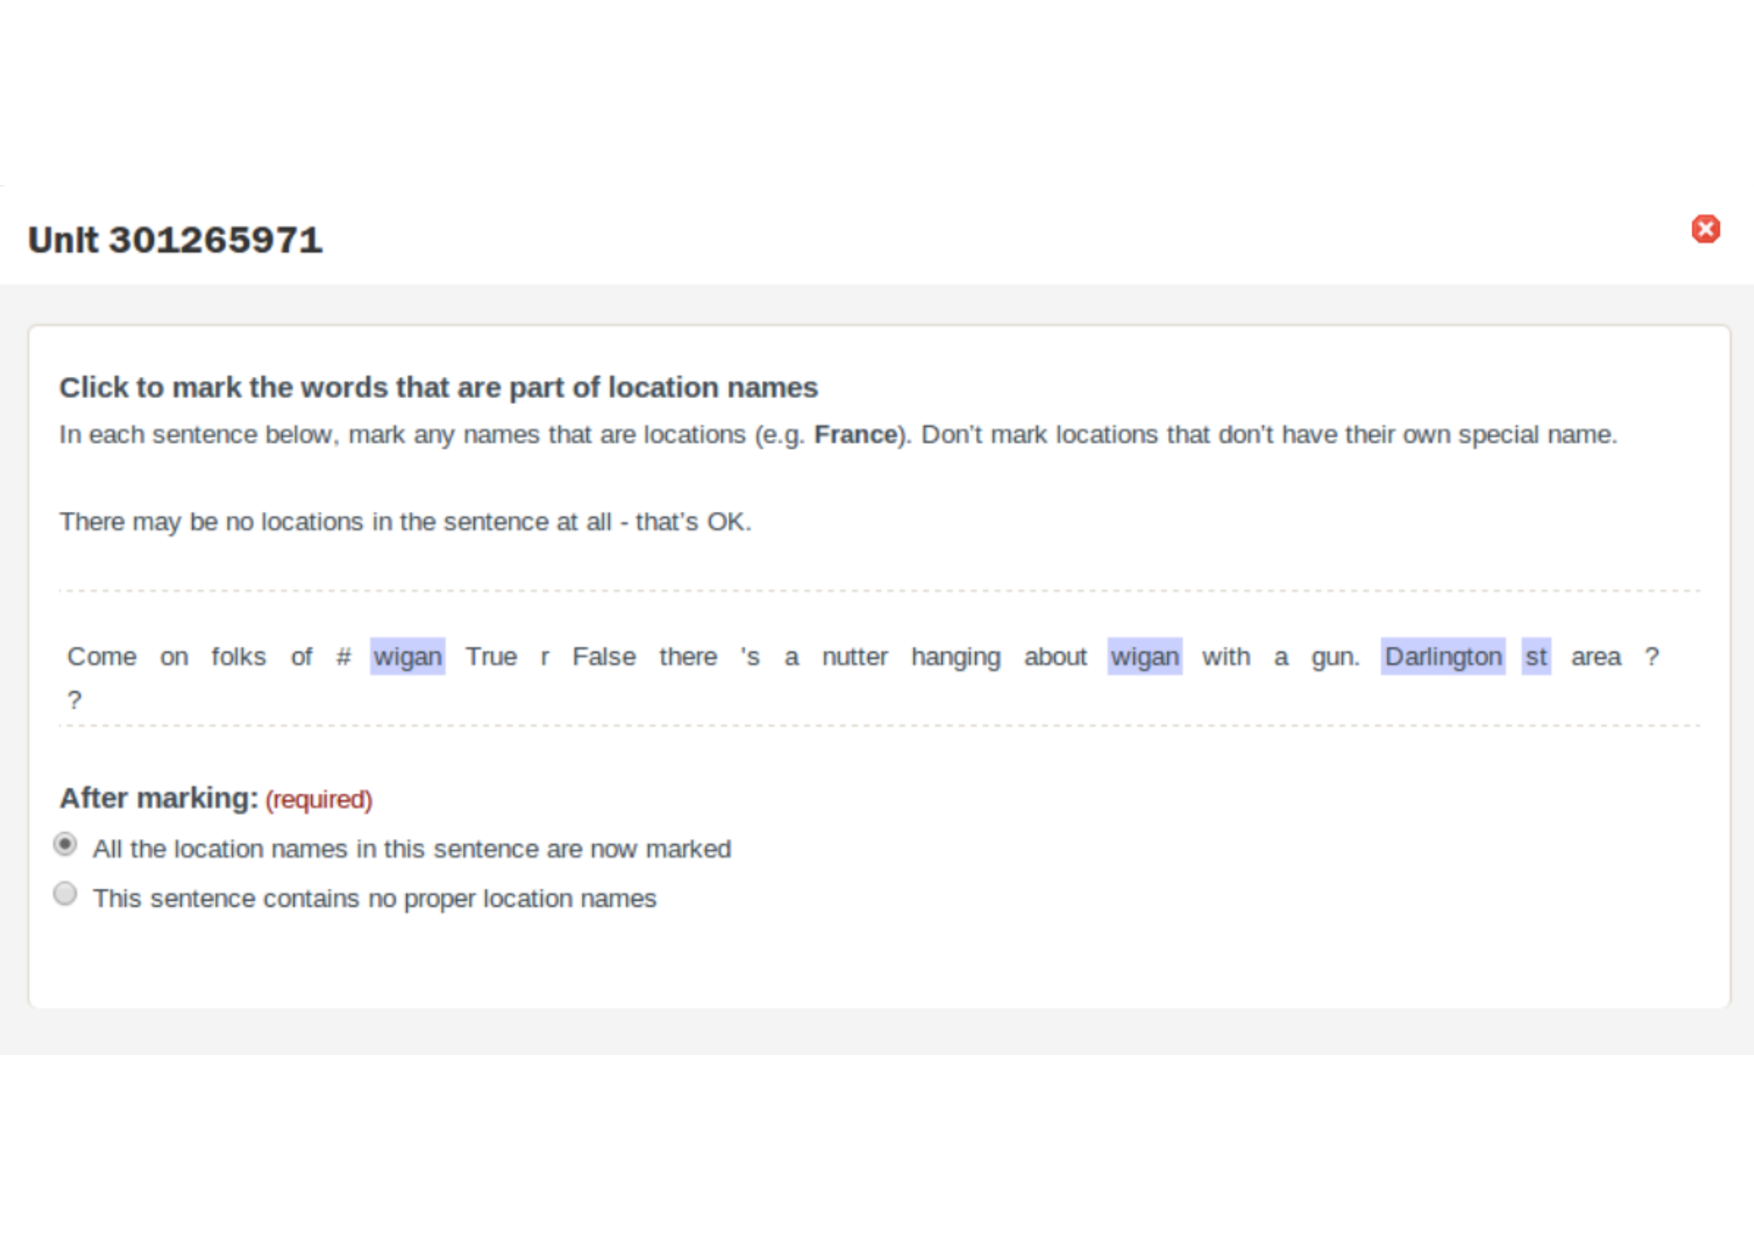
\includegraphics[width=0.75\textwidth]{graphics/named_entity_recognition}
	 \caption{Crowdsourcing task interface for named entity recognition~(adopted from~\cite{bontcheva2017})}
	 \label{fig:named_entity_recognition}
\end{figure}  
After identifying the named entities, the next step is entity linking to find potentially ambiguous entities. DBpedia~\cite{auer2007} was chosen as target entity linking database because of its good coverage of named entities, its frequent updates and available mappings to other Linked Data sources. 


\paragraph{Data Storage and Indexing} 
Up to this stage, the data was already mapped to the \gls{rdf} data model but needs to be stored and indexed efficiently. Researchers have put a lot of effort into this field because efficient storage and indexing mechanisms are fundamental for the adoption of Linked Data. Due to efficient querying and storage capabilities of relational databases resulting from decades of research in this area, it makes sense to adopt these approaches for Linked Data as well~\cite{abadi2007}. However, to support storing very large quantities of data there exist custom solutions too~\cite{broekstra2002}. Targeting Linked Data indexing, various approaches and principles have been applied successfully. The common aspects of all approaches is their focus on \emph{Data Compression} and \emph{Data Pruning}~\cite{svoboda2011}. Whereas the basic idea of Data Compression is to minimise the footprint of the index, Data Pruning is a technique for avoiding unnecessary data processing. 

%Crowdsourcing example LED \cite{adamou2014}%
Whereas Data Indexing is traditionally done solely by machines, there are some approaches that combine Crowdsourcing and Semantic principles for Data Storage. One of them is the \gls{led}\footnote{\url{https://led.kmi.open.ac.uk/} accessed 2019/04/01}, a semantic knowledge base of accounts of listening to music in documented sources~\cite{adamou2014}. \gls{led} stores listening evidences of music across history and musical genres. Its dataset includes more than \numprint{10000} entries collected from various sources, volunteers from the crowd being one of them. 

\paragraph{Data Revision and Authoring} In this stage users are given the opportunity to create new or modify existing semantic information. 
This is called \textit{\gls{sca}} which is defined in the literature as~\textit{"a tool-supported
manual composition process aiming at the creation of semantic documents."}~\cite{khalili2013} More generally speaking, \gls{sca} is actually embedded in a broader ecosystem for semantic content authoring as shown in~\hyperref[fig:authoring_semantic_ecosystem]{Figure~\ref*{fig:authoring_semantic_ecosystem}}. 
\begin{figure}
	 \centering
	 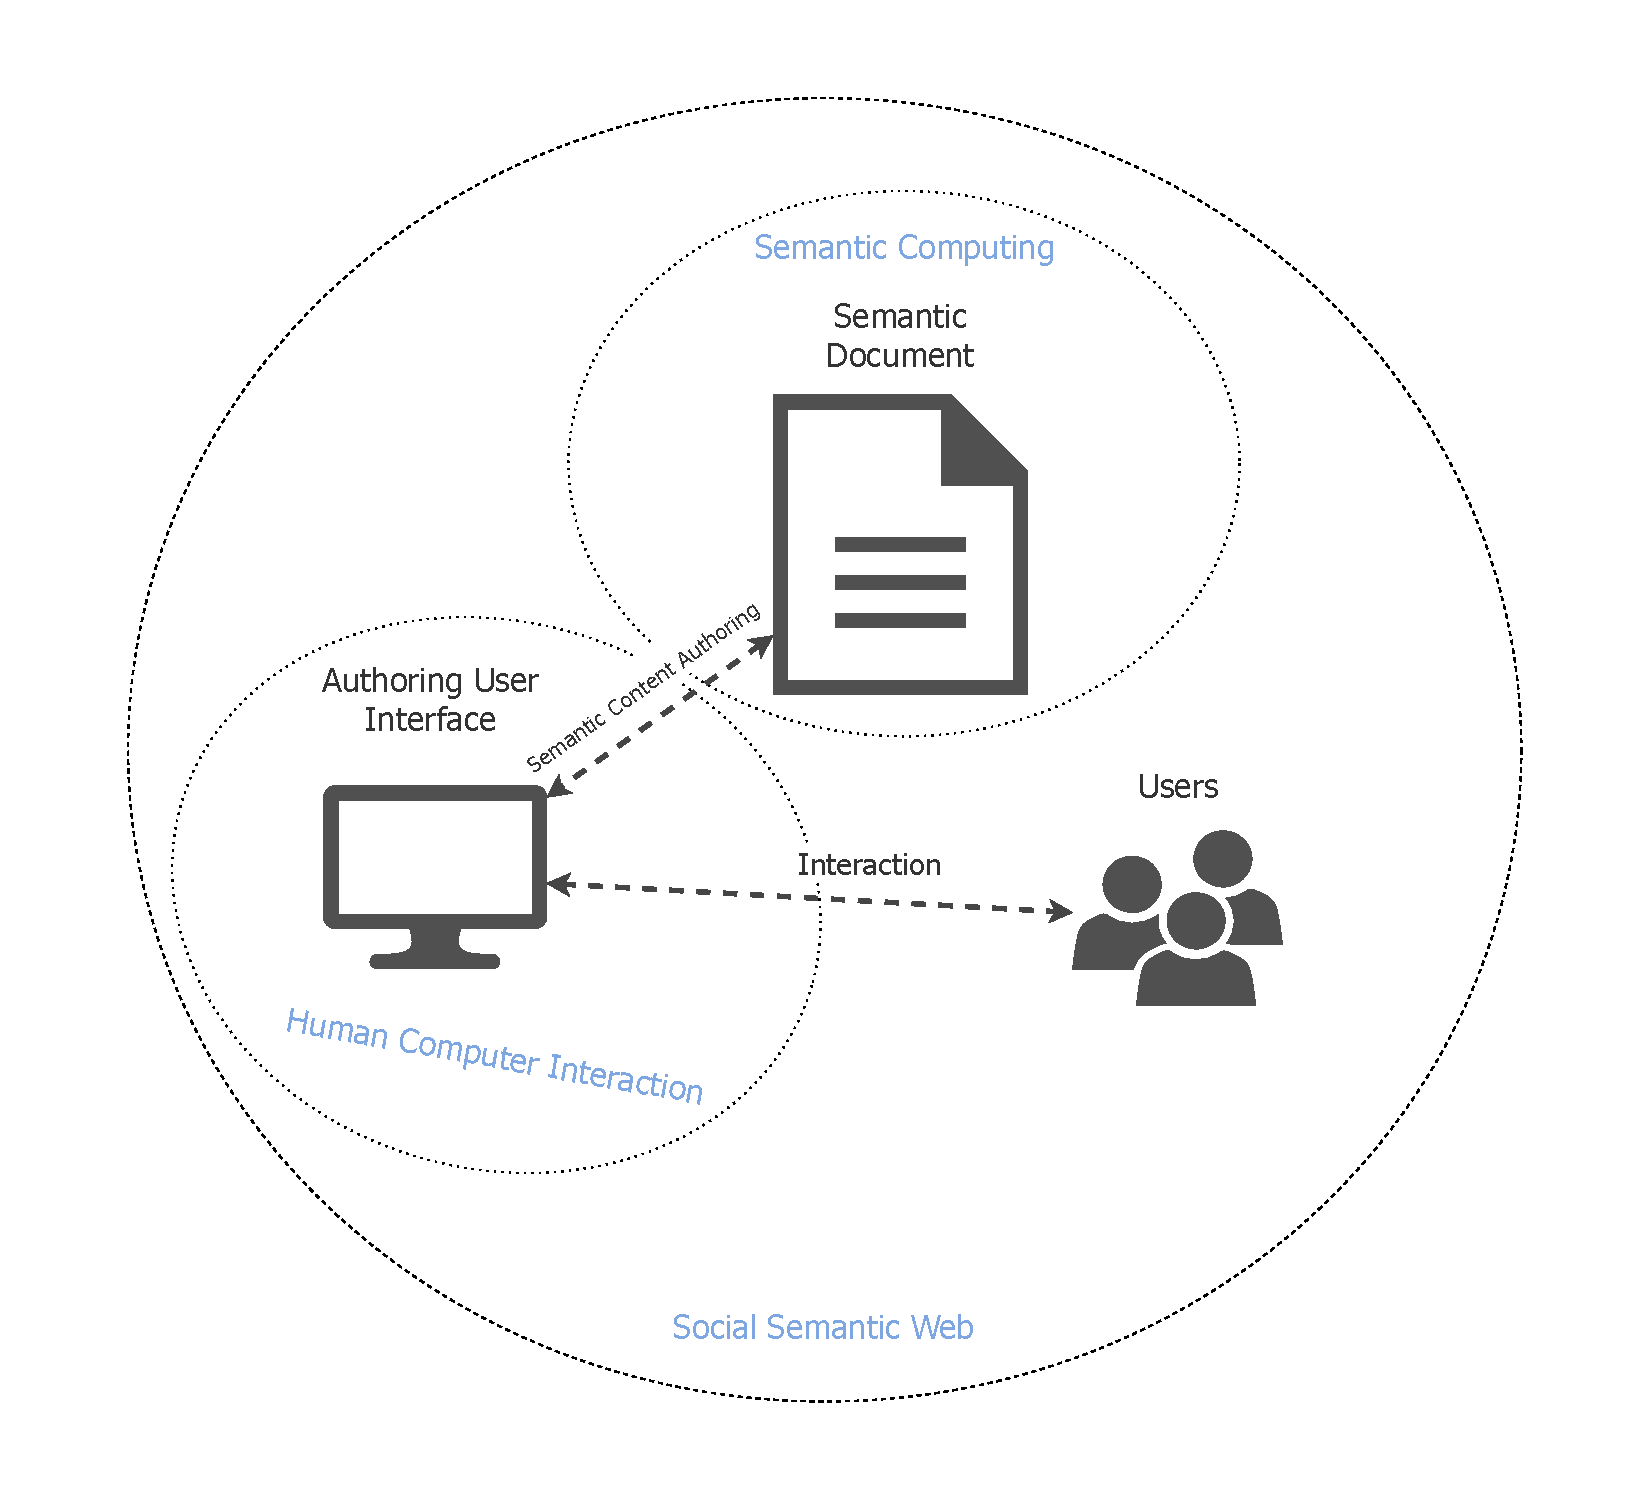
\includegraphics[width=1\textwidth]{drawio/authoring_semantic_ecosystem}
	 \caption{The ecosystem for semantic content authoring}\label{fig:authoring_semantic_ecosystem}
\end{figure}
The central entity of the semantic ecosystem is a semantic document which holds semantically enriched information. 
In information management, semantic documents serve a number of purposes such as information searching, information retrieval, information presentation, information integration, personalisation, reusability and interoperability~\cite{khalili2013}. For that reason there exists a research area dealing with the main fields of semantic content management. In particular, it covers the manipulation, creation and processing of semantic content. Users do not directly interact with semantic documents, but rather through a uniform \gls{ui}. A number of quality attributes for the assessment of \gls{ui}-features of \gls{sca}-Systems were proposed~\cite{khalili2013}. The goal was to improve usability, a measure of the effectiveness, efficiency and satisfaction a user achieves. 

%Crowdsourcing example Mechanical Protege \cite{simperlMechnicalProtege}%
A number of tools for semantic content authoring were developed. A good example that adds Crowdsourcing capabilities to ontology development activities is Mechanical~Protege~\cite{simperlMechnicalProtege}. The tool is a plug-in for the ontology editor Protege\footnote{\url{https://protege.stanford.edu/} accessed 2018/08/07}. It allows creating classification hierarchies or labelling concepts and translating them into different languages. The user can choose from a set of pre-configured tasks, adjust parameters such as task description or reward for crowd workers and create Crowdsourcing jobs for Amazon~Mechanical~Turk\footnote{\url{https://www.mturk.com/} accessed 2019/04/03}. In the example shown in~\hyperref[fig:mechanical_protege_example]{Figure~\ref*{fig:mechanical_protege_example}} the user created a task to translate English labels into German labels for the concepts \emph{Spiciness}, \emph{Medium}, \emph{Hot}, \emph{IceCream}, \emph{Pizza} and \emph{PizzaBase}. Furthermore, settings were adjusted to require 2 judgements for each concept and paying crowd workers $0.05$ \$ for task completion.  
\begin{figure}
	 \centering
	 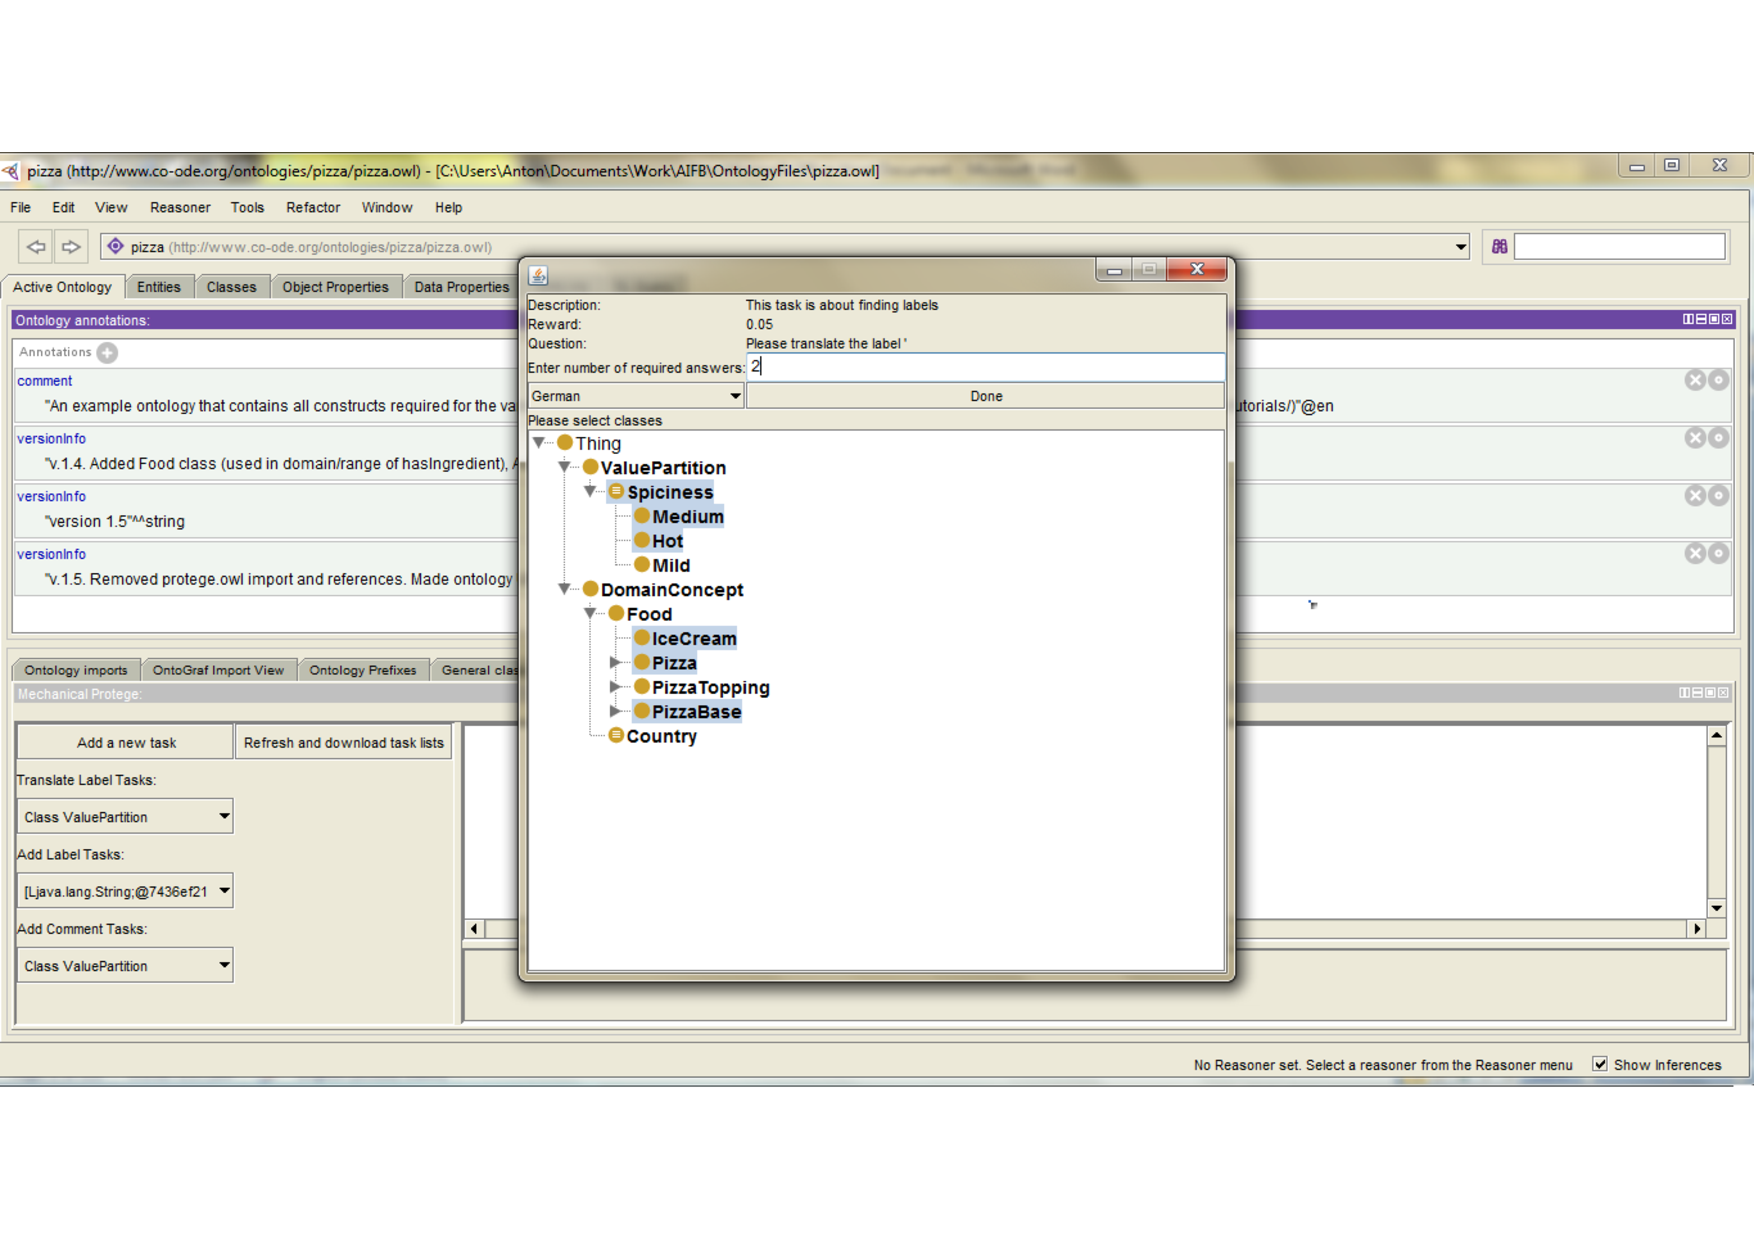
\includegraphics[width=1\textwidth]{graphics/mechanical_protege_example}
	 \caption{Crowdsourcing task creation in Mechanical Protege for translating concept labels}
	 \label{fig:mechanical_protege_example}
\end{figure}

\paragraph{Data Linking}
The next principle according to the Linked Data Life-Cycle is the Data Linking principle. It is by far the most important principle because it 
underlines the distributed nature of Linked Data. Instead of the traditional definition of data where information is stored in silos with little or no relations to the outside, Linked Data sources are distributed, containing many links to other data sources. This paradigm perfectly fits into the distributed nature of the Web, turning it into a source of distributed information optimised for querying and browsing. 

%Crowdsourcing example ZenCrowd~\cite{demartini2012}%
Using automated techniques of entity linking can be quite challenging, since parsing and disambiguating natural language
text is considered a difficult task when done algorithmically. The process of relating entities extracted from text to their equivalents in the Linked Data space can be done automated~(\emph{Algorithmic Matching}) or with human intervention~(\emph{Manual Matching}). ZenCrowd~\cite{demartini2012} combines those two approaches by first trying the algorithmic approach and then improving the results by involving human workers. The main steps of the linking process are shown in~\hyperref[fig:zencrowd]{Figure~\ref*{fig:zencrowd}}.
\begin{figure}
	 \centering
	 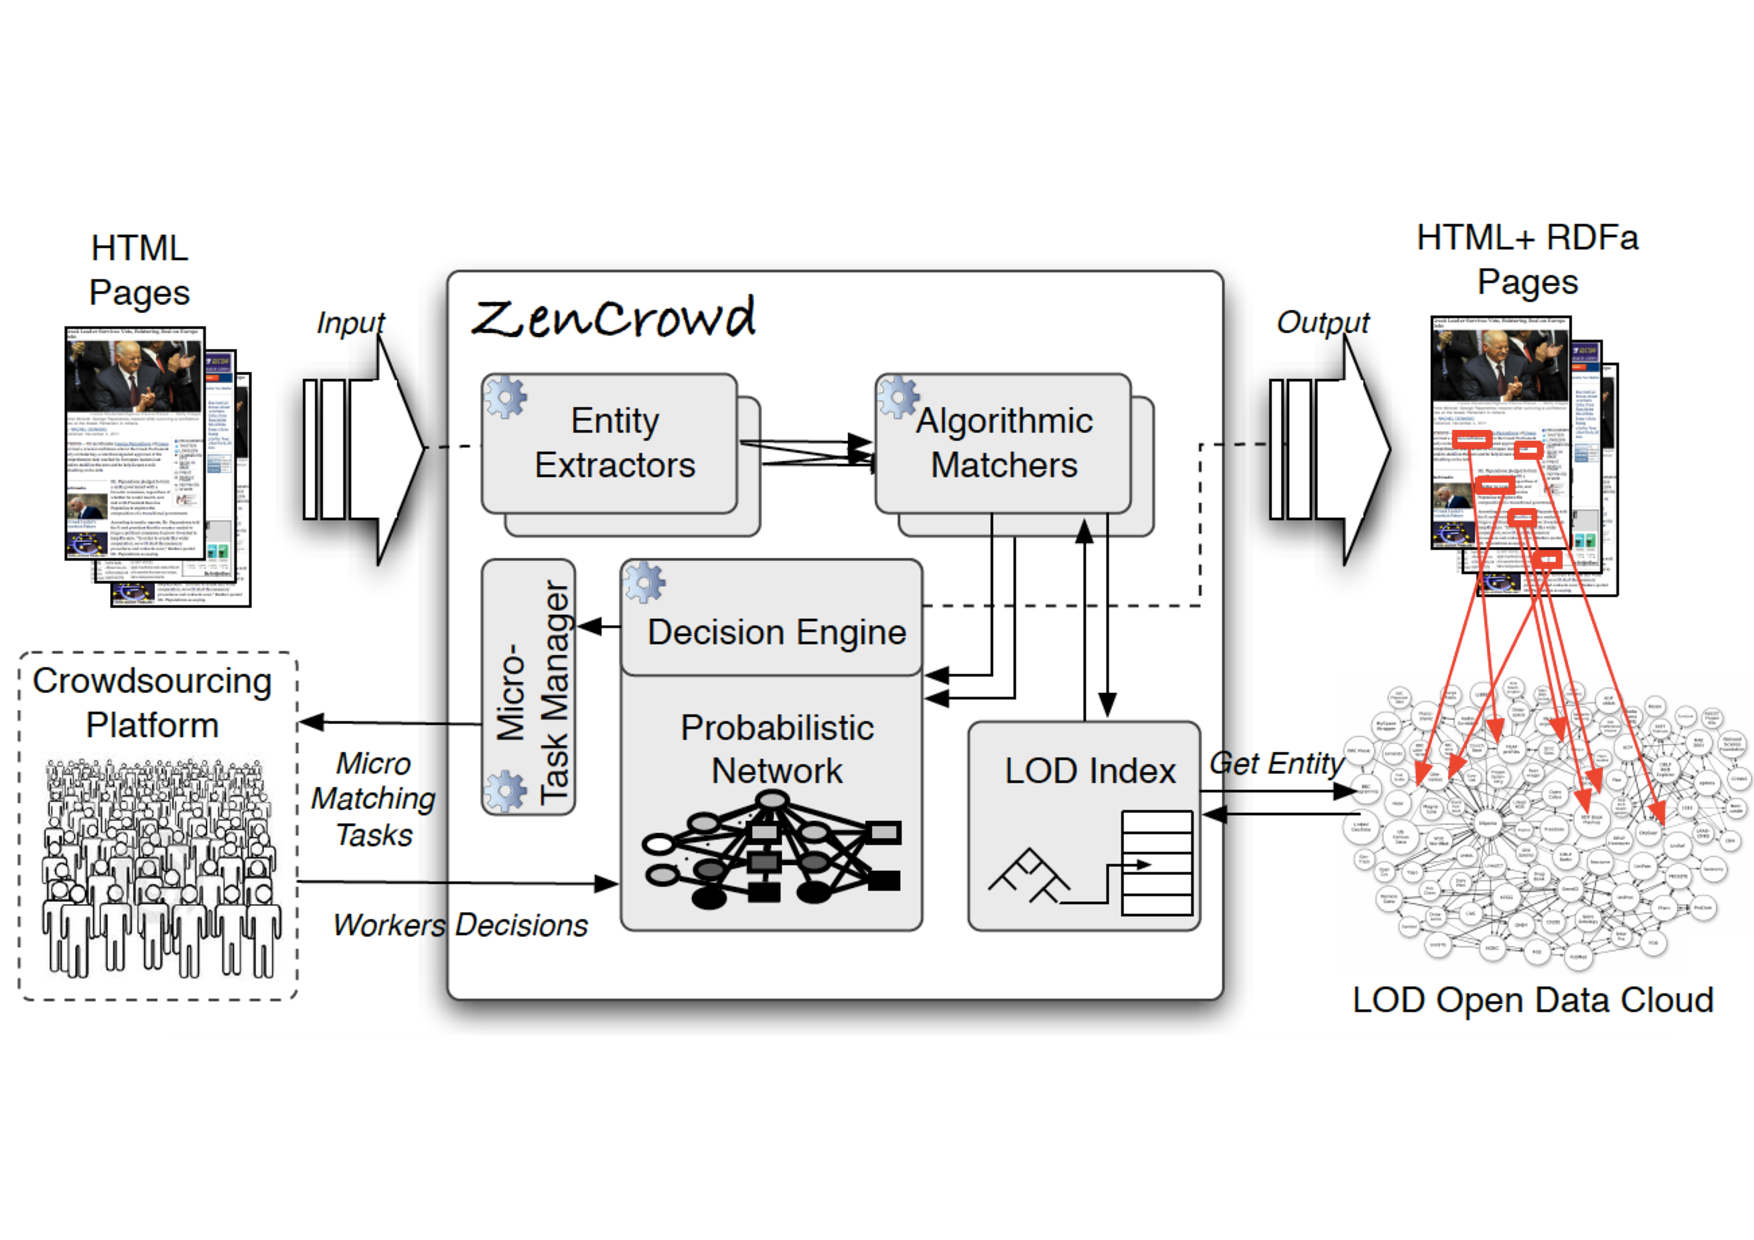
\includegraphics[width=\textwidth]{graphics/zencrowd}
	 \caption{The linking process of ZenCrowd~(adopted from~\cite{demartini2012})}
	 \label{fig:zencrowd}
\end{figure}
The process takes as input a collection of HTML pages. Those pages were then inspected by the \emph{Entity Extractors} to detect relevant textual entities. In the next step \emph{Algorithmic Matchers} try to create links to semantically similar entities from the linked data set. The results of this process are stored in a \emph{Probabilistic Network} which is taken by the \emph{Decision Engine} to decide whether the results are useful or not. In the latter case, the HTML pages are passed to the \emph{Micro-Task Manager} which uses Crowdsourcing to improve the results. 


\paragraph{Classification and Enrichment}
Over time, Linked Data sources grow in size and expressiveness. This principle refers to the process of extending the expressiveness and richness 
of semantic knowledge bases. It means that instead of creating the structure upfront, the knowledge base evolves over time. For that, the knowledge 
base is typically enriched by analysing existing data to improve or extend its schema. A variety of (semi-)~automatic enrichment approaches emerged over the past years. The methods span across several research areas, including machine learning, statistics, natural language processing, to name just a few. 

%Crowdsourcing exmaple \cite{wohlgenannt2013}%
Even though automating the process of ontology refinement greatly reduces the need for expert contribution, there are still some tasks which require human involvement. \cite{wohlgenannt2013} presented a model for evolving lightweight ontologies and a prototype which implements the model. The model describes the ontology learning process which uses Crowdsourcing to validate the concepts of the learned ontology. The algorithmic part of the process takes a seed ontology as input which is then continuously extended. This process is repeated until the target ontology reflects the semantics of the input source. The prototypical implementation only accepts textual input sources but future adaptations were planned. 
For the Crowdsourcing part a \gls{gwap} is used to eliminate unrelated concepts. The players of the game had to analyse the concept's relevance to the ontology's domain. The results of the Crowdsourcing part were taken to improve the quality of the learned ontology. 

\paragraph{Data Analysis and Quality}
Due to the distributed nature of Linked Data where information originating from heterogeneous data sources is merged, the quality of the resulting
dataset is often varying. Therefore, a key factor for the adoption of Linked Data is ensuring its quality by identifying and fixing common problems. Before that, it is necessary to determine the quality of the existing dataset. For that, metrics which measure the quality in terms of accuracy, completeness, adequacy and degree of understandability need to be defined. \cite{zaveri2016} defines useful quality metrics along with 26 quality dimensions that help to measure the quality of the Linked Data.

%Crowdsourcing example \cite{mortensen2015}%
In~\cite{mortensen2015} the authors analysed 200 taxonomic relations of SNOMED~CT, a widely used ontology mainly used in biomedical contexts. They used Crowdsourcing to detect inconsistencies and address the challenges of scalable ontology verification. The Crowdsourcing task interface shows the description of the evaluated relation and set of related concept definitions. The crowd worker can then either agree~(by answering \emph{yes}) or disagree~(by answering \emph{no}) on the presented statements. 


\paragraph{Data Cleansing and Evolution}
After the quality is analysed and problems are detected, strategies for fixing these problems are needed. In constantly evolving datasets with millions or even billions of \gls{rdf} triples it is important to keep the links between datasets. Likewise, conflicts and discrepancies in datasets can cause real trouble. Repairing such inconsistencies in overlapping datasets is called \emph{Data Fusion}. Several works focusing on repairing problematic datasets appeared in the literature. For example, \cite{mendes2012} considers repairing with respect to data fusion and \cite{flouris2012} investigates how provenance helps to improve the quality of Linked Data. In this context, provenance refers to where and how the data was obtained from. 

%%Crowdsourcing example uComp Protege Plugin~\cite{wohlgenannt2016}%%
The uComp Protege Plugin~\cite{wohlgenannt2016} is a good example which combines Data Cleansing and Crowdsourcing. An in-depth explanation is out of scope for this section. However, a detailed description of the plugin is given in~\hyperref[sec:ucomp_protege_plugin]{Section~\ref*{sec:ucomp_protege_plugin}} as it represents the baseline of this thesis.
As soon as the results from the crowdsourced ontology validation are available, the plugin guides the user to take further actions as summarised in~\hyperref[table:data_cleansing_ucomp_protege]{Table~\ref*{table:data_cleansing_ucomp_protege}}. For each task the user can take advantage of the following cleansing actions: \emph{Concept Removal} for the Verification of Domain Relevance, \emph{Relation Removal} for the Verification of Relation Correctness, \emph{Relation Labelling} for the Specification of Relation Type and \emph{Domain/Range Removal} for the Verification of Domain/Range. 
\begingroup
\renewcommand{\arraystretch}{2}
	\begin{table}
		\centering
		\begin{tabularx}{0.8\textwidth}{l l}
			\toprule
			Task Type & Cleansing Action \\
			\midrule
	        Verification of Domain Relevance & Concept Removal \\
			Verification of Relation Correctness & Relation Removal \\
			Specification of Relation Type & Relation Labelling \\
			Verification of Domain and Range & Domain/Range Removal \\
			\bottomrule
		\end{tabularx}
		\caption{Data Cleansing capabilities of the uComp Protege Plugin}
		\label{table:data_cleansing_ucomp_protege}
	\end{table}
\endgroup


\paragraph{Data Browsing and Querying}
Last, users have the opportunity to explore the Linked Data available on the Web in a fast and efficient way. A prominent way to query Linked Data is
\gls{sparql}\footnote{\url{https://www.w3.org/TR/rdf-sparql-query/} accessed 2019/01/17}, a query language specifically designed to retrieve and manipulate Linked Data. There are similarities between \gls{sql} and \gls{sparql} in terms of query structure, but there are also differences.

%Crowdsourcing example LexiTags~\cite{veres2013}%
LexiTags~\cite{veres2013} is an example which combines Semantic Browsing and Crowdsourcing. It was initially designed as a tool for content management and emerged to a platform that expose crowdsourced semantic metadata to clients, both for creation and consumption of metadata. Its main interface keeps a list of bookmarked URLs, allowing users to add and edit semantic tags. Semantic tagging is a very powerful innovation which helps users to navigate through large datasets by constructing search queries from a set of semantic tags. 

